% -*- mode: noweb; noweb-default-code-mode: R-mode; -*-
\documentclass[a4paper]{article}
%\VignetteIndexEntry{RiboSort User Manual}
%\VignetteDepends{RiboSort}
%\VignetteKeyword{RiboSort}
\usepackage{graphicx}
%Redefining the internal command fps@figure from it's default tbp to what I want the default to be:htp
\makeatletter
\def\fps@figure{htp}
\makeatother
%\setlength{\textheight}{8in} % height of main text
%\setlength{\textwidth}{6in}    % width of text


\title{RiboSort User Manual}
\author{\'{U}na Scallan}

\usepackage{C:/R-2.4.1/share/texmf/Sweave}
\begin{document}

\maketitle

\section {Introduction}

RiboSort is an R package for automated data preparation and exploratory analysis of microbial community profiles. It facilitates the sorting of many automatic sequencer generated profiles at once, thus eliminating the tedious and time consuming operation of manually manipulating and sorting profiles. 

This document illustrates a sample session using the RiboSort package. It goes through loading data, running \texttt{RiboSort} to sort the data, and manipulating results for preliminary statistical analysis. We assume a basic  knowledge of R, and thus advise familiarization with Appendix 1: Getting Started in R, if this is your first encounter with the R programming environment.

To begin, start R, then load the RiboSort package:

\begin{Schunk}
\begin{Sinput}
> library(RiboSort)
\end{Sinput}
\end{Schunk}
\section{Data Retrieval}

RiboSort facilitates the direct input of data produced by two automatic sequencers, the Applied Biosystems (ABI) Gene Mapper and the Beckman Coulter CEQ 8000 Genetic Analysis System. Data can also be read from other formats if you reformat it manually into RiboSort's defined standard profile (see section~\ref{sec:std}). We welcome contributions for routines for importing data from other formats.

\subsection{\textbf{Standard Profile}}
\label{sec:std}
A standard profile defined for the RiboSort package contains two columns. The first column lists fragments detected in the sample in increasing order. Their associated relative abundances, represented by peak heights in the sequencer output, are listed in a second column. An example of a standard profile is illustrated in Figure~\ref{fig:std}.

\begin{figure}
\centering
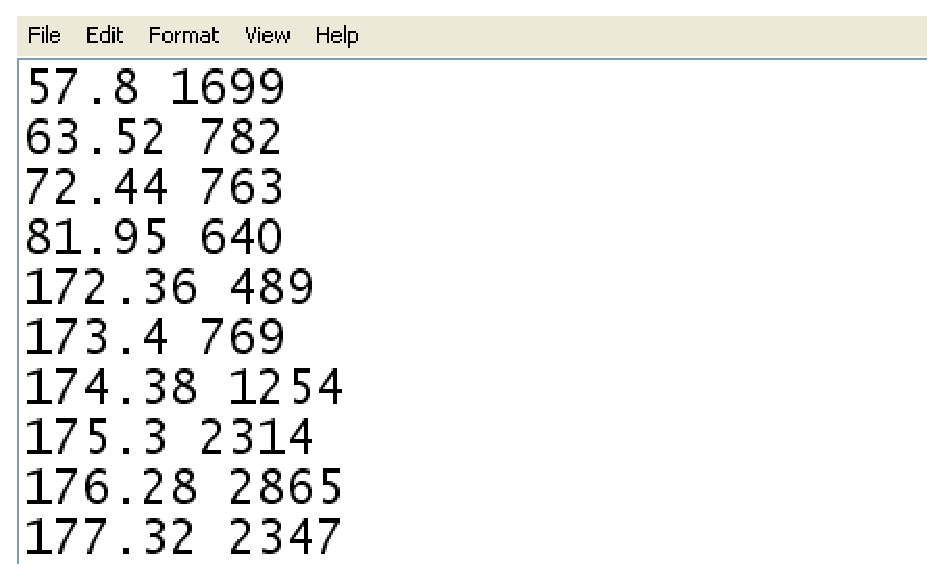
\includegraphics[width=0.5\textwidth,height=1in]{EPS/picstandard.eps}
\caption{RiboSort's standard profile format.}
\label{fig:std}
\end{figure}

\subsection{\textbf{Applied Biosystems 3130XL (GeneMapper)}}
The ABI 3130XL sequencer and its associated GeneMapper version 4.0 software allow data to be exported in a wide variety of formats. Two of these formats are compatible with RiboSort. The first contains a single community profile which we  denote ABIsingle, and the second can contain multiple profiles, denoted ABImultiple. Instructions for retrieval of these formats using the GeneMapper software are now described.
\newline
\newline
\textbf{ABIsingle}

\begin{itemize}
\item Once logged into the GeneMapper software, select {\em File $\rightarrow$ Open}  project from the top menu. Highlight the desired project and click on Open. Set tablesettings to AFLP default.
\item Proceed by highlighting the sample to be exported. Click on the Display Plot icon in the top toolbar. In the plot window that opens, set plot settings to sizing, and subsequently select {\em File $\rightarrow$ Export table}. Save the text file under its sample name in the desired location.
\item An example of such a file is illustrated in Figure~\ref{fig:abisingle}.

\begin{figure}
\centering
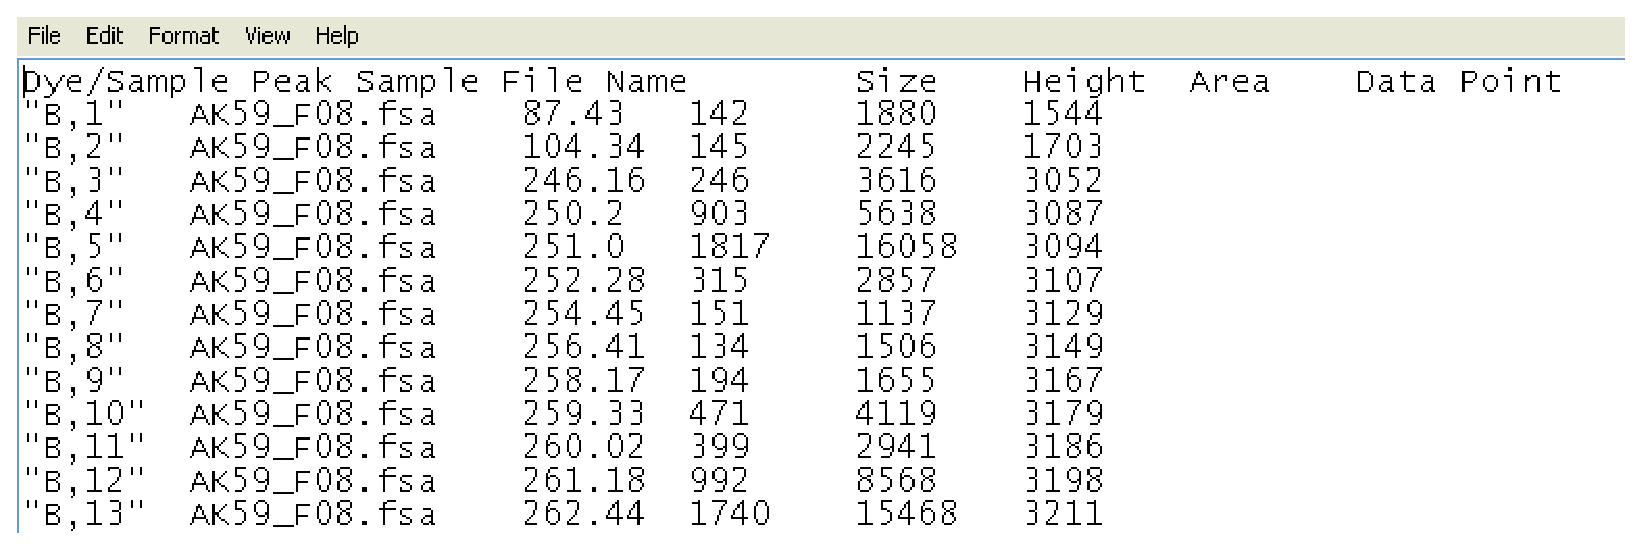
\includegraphics[width=0.8\textwidth,height=1.5in]{EPS/picabisingle.eps}
\caption{An ABIsingle text file.}
\label{fig:abisingle}
\end{figure}

\end{itemize}
\textbf{ABImultiple}

\begin{itemize}
\item Once logged into the GeneMapper software, select {\em File $\rightarrow$ Open} from the top menu. Highlight the desired project and click on Open. Set tablesettings to AFLP default.
\item Open the Genotypes tab and take note of the maximum allele number detected in the set of samples. From the top menu, select {\em Tools $\rightarrow$ GeneMapper Manager}. Open the Report Settings tab and enter the project name into the space provided. The maximum allele number should be entered into the Number of Alleles box.
\item In the Genotype tab of the Available Columns box, highlight the fields to be included in your output (these are sample name, all sizes and all heights) and click on the arrow pointing right toward the Selected Columns box. Click on OK.
\item  Back in the GeneMapper window, highlight the samples you wish to export, or if all samples are to be included in the output file, enter {\em Edit $\rightarrow$ Select all}.
\item On the top menu, enter {\em Analysis $\rightarrow$ Report Manager}. In the report manager window that opens, there is a drop-down menu entitled Report Settings. In this menu, select the project you just created.
\item On the top menu, select {\em Edit $\rightarrow$ Flip Table}. Then select {\em File $\rightarrow$ Export\ldots} and save the output text file under its project name in the desired location. An example of such a file is illustrated in Figure~\ref{fig:abimulttxt}.

\begin{figure}
\centering
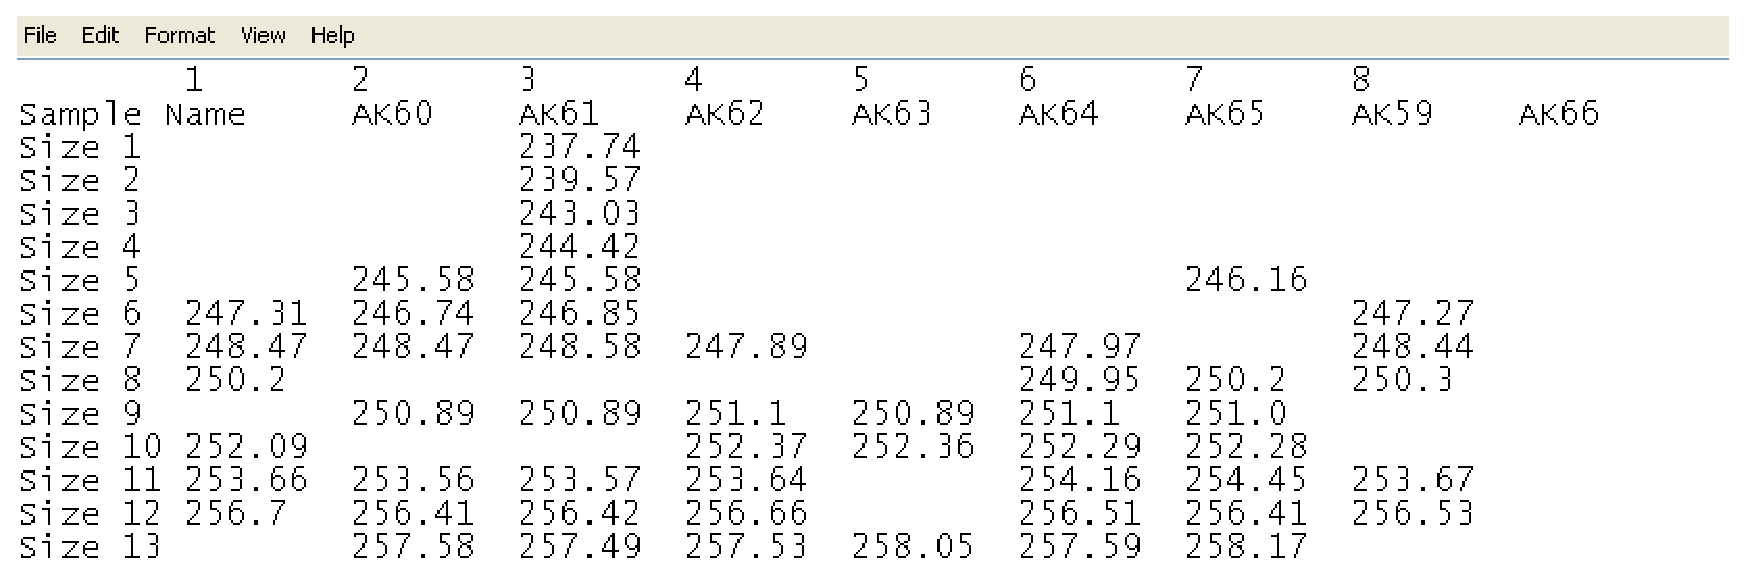
\includegraphics[width=0.8\textwidth,height=1.5in]{EPS/picabimultipletxt.eps}
\caption{An ABImultiple text file.}
\label{fig:abimulttxt}
\end{figure}

\item One final step is required to make this output compatible with RiboSort. Open the text file, say projectname.txt, in Excel. Select {\em File $\rightarrow$ Save as\ldots} and save the file as a comma separated file, projectname.csv. This file is now ready to be used in the RiboSort package. An example of such a file is illustrated in Figure ~\ref{fig:abimultcsv}.

\begin{figure}
\centering
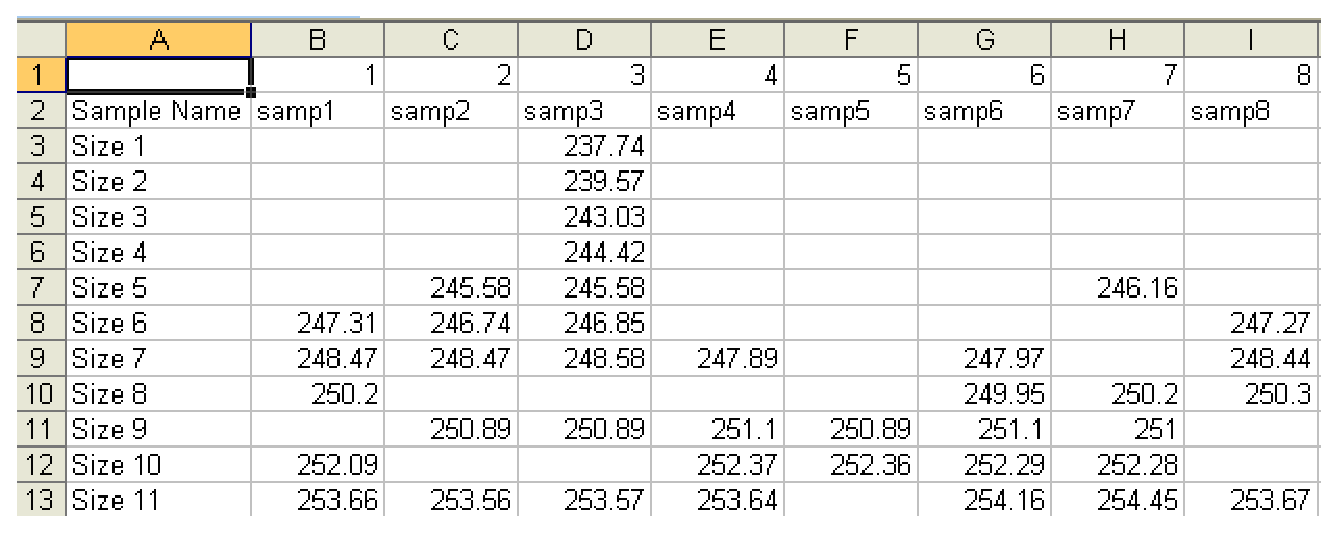
\includegraphics[width=0.8\textwidth,height=1.5in]{EPS/picabimultiplecsv.eps}
\caption{An ABImultiple comma separated file.}
\label{fig:abimultcsv}
\end{figure}

\end{itemize}
Note: Ensure that no empty profiles are exported to the text file created by GeneMapper. An empty profile containing no sequencer detections will make the text file incompatible with RiboSort and will produce an error if submitted. 
\subsection{\textbf{Beckman Coulter CEQ 8000 Genetic Analysis System}}
The CEQ 8000 control and analysis software allows data to be exported in a wide variety of formats. To retrieve analysis results in a RiboSort compatible format, follow the guidelines given below.
\begin{itemize}
\item Open the Genetic Analysis System software and from the top menu in the sequencer program, select {\em File $\rightarrow$ Export Results}.
\item Choose the sample to be exported and proceed, leaving all default settings in place. On the Elements page, ensure that the \textit{Header} and \textit{Results Data} options are not ticked. This action will create a RiboSort compatible text file.
\item  An example of such a file is illustrated in Figure~\ref{fig:beckman}.

\begin{figure}
\centering
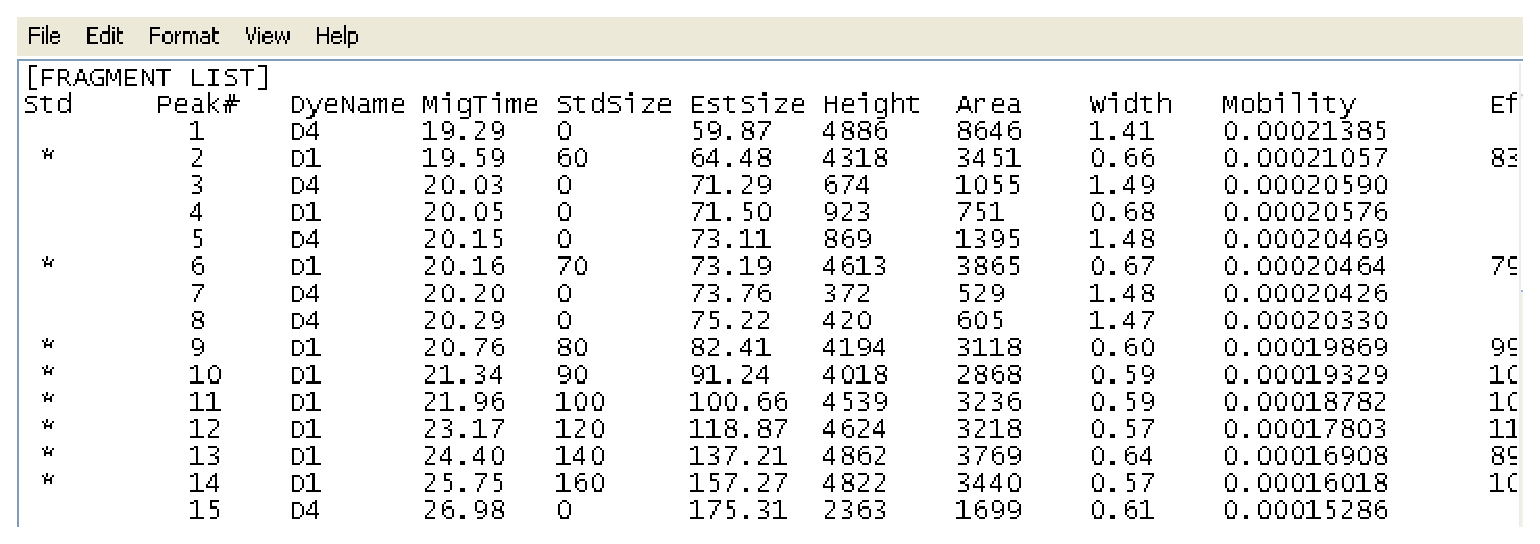
\includegraphics[width=0.8\textwidth,height=1.5in]{EPS/picbeckman.eps}
\caption{An extract from a Beckman text file.}
\label{fig:beckman}
\end{figure}

\end{itemize}


\section{Data Loading}

To load data for use with the RiboSort package, copy any data files to be sorted into your current working directory (see Appendix 1 for explanation of the working directory). The RiboSort package contains a number of R functions. The behaviour of these functions can be altered by changing optional arguments. The most important function in this package is \texttt{RiboSort} itself. This is the function to which you submit your data. In order to submit more than one file at a time to the \texttt{RiboSort} function, a data vector containing the list of filenames needs to be created. We now demonstrate how to create a data vector called \texttt{mydata} in R.

\begin{Schunk}
\begin{Sinput}
> mydata = c("sample1.txt", "sample2.txt", "sample3.txt", "'sample4.txt")
\end{Sinput}
\end{Schunk}
There is a limit of 1000 characters allowed for filenames within the parentheses of a data vector. When there are many files to be processed and the character limit in \texttt{mydata} is reached, successive files can be stored in additional datasets \texttt{mydata2}, \texttt{mydata3}, etc. All datasets can then be combined into a total data vector as shown in the example below. 

\begin{Schunk}
\begin{Sinput}
> mydata1 = c("sample1.txt", "sample2.txt", ..., "sample74.txt")
> mydata2 = c("sample75.txt", "sample76.txt", ..., "sample149.txt")
> mydata3 = c("sample150.txt", "sample151.txt")
> allmydata = c(mydata1, mydata2, mydata3)
\end{Sinput}
\end{Schunk}
In this example the data vector that should be submitted to the \texttt{RiboSort} function is \texttt{allmydata}. Note that with the exception of ABImultiple files, which are comma separated (\textit{.csv}), all other data files will be text files (\textit{.txt}). It is also important to note that all files listed in a data vector must be of the same format (either Standard, ABIsingle, ABImultiple or Beckman).

\section{The RiboSort Function}

Depending on the size and number of  data files, and the speed of your computer, running \texttt{RiboSort} may be slow. There are seven arguments to the function \texttt{RiboSort}. Each of these arguments works as a interactive tool, allowing the user to personalize the method of classification carried out. See the help file \texttt{?RiboSort} for more information. To run the examples in the help file, all the demonstration datafiles (including thirteen \textit{.txt} files and one \textit{.csv} file) provided in the RiboSort package must be copied to your current working directory. 

The complete \texttt{RiboSort} function is shown below, with each of the seven arguments set to their default values.

\begin{Schunk}
\begin{Sinput}
> x = RiboSort(data, dataformat = "standard", dye = "B", output = "proportions", 
+     zerorows = FALSE, repeats = 1, mergerepeats = "none")
\end{Sinput}
\end{Schunk}
We now proceed to describe the purpose of each argument and the available options for them.

\begin{description}
  \item[\texttt{data}] A data vector listing the filenames of each profile to be sorted. Recall that each file listed must be stored in the current working directory to be detectable by R.
  \item[\texttt{dataformat}] The format of profiles listed in \texttt{data}. This must be one of \texttt{"standard"},  \texttt{"abisingle"}, \texttt{"abimultiple"} or \texttt{"beckman"}.
  \item[\texttt{dye}] An indicator code identifying the dye that corresponds to the primer used. The argument \texttt{dye} only comes into effect when \texttt{dataformat} is \texttt{"abisingle"} or \texttt{"beckman"}. The ABIsingle files generally just have a single letter dye indicator, eg. \texttt{"B"}, \texttt{"R"}, \texttt{"Y"}, etc., whereas Beckman sequencer files usually have dye indicators of the form \texttt{"D1"}, \texttt{"D4"}, etc.
  \item[\texttt{output}] Specifies whether the R object produced by RiboSort will contain abundances (as given in the original profiles) or the relative proportions of abundance in each profile. \texttt{output} must be one of \texttt{"abundances"} or \texttt{"proportions"}. Statistical analysis is usually performed on the relative proportions of abundance, thus the default is \texttt{"proportions"}. 
  \item[\texttt{zerorows}] A logical argument (can only take values \texttt{TRUE} or \texttt{FALSE}) indicating whether zerorows are to be kept in the output or not. A zerorow refers to a ribotype not detected in any of the profiles supplied. When \texttt{FALSE}, the default, zerorows are deleted from the output. When \texttt{TRUE}, the zerorows remain in the output.
  \item[\texttt{repeats}] The number of repeat profiles taken from each sample. If \texttt{repeats} is greater than 1, profiles listed in \texttt{data} must be in an order, such that all repeats from a particular sample are listed adjacent to one another. For example, if there were two repeats and five samples, Samp1repeat1 would be listed first followed by Samp1repeat2, Samp2repeat1, Samp2repeat2, etc.
  
The number of repeats must be constant for all samples. If this is not the case, submit \texttt{repeats = 1} to obtain a sorted output of all profiles, and proceed to manually merge repeat profiles.
  \item[\texttt{mergerepeats}] The method of merging a number of repeat profiles from the same sample into a single composite profile for that sample. \texttt{mergerepeats} must be one of \texttt{"none"}, \texttt{"presentinall"}, \texttt{"presentintwo"} or \texttt{"presentinone"}.
  
The \texttt{"none"} option indicates that profiles are not to be merged. To merge repeat profiles taken from the same sample into a single composite profile, there are three methods. The first of these, \texttt{"presentinall"}, specifies that the composite profile only contains ribotypes detected in all of the repeat profiles. Thus, ribotypes present in less than all of the repeat profiles, are not included in the final composite profile. 

The second method, \texttt{"presentintwo"}, specifies that the composite profile only contain ribotypes detected in at least two of the repeat profiles. Finally, the \texttt{"presentinone"} method indicates that all ribotypes detected, even those only present in one repeat profile, are included in the composite profile. This is the default option.

Following the execution of any of the three merging methods, the composite profile produced for a sample will be named according to the first repeat profile listed in \texttt{data} for that sample.

Composite profile abundances are determined by averaging the relative proportions present in repeat profiles.

When \texttt{repeats} is greater than 1 and  \texttt{mergerepeats="none"}, no profile merging will occur and all profiles submitted will be present in the output.

\end{description}

\section{Managing and Saving Output}
Each time the RiboSort function is run, four Excel files are created and stored in the current working directory. {\em Ribotypes Output.xls} contains assigned and aligned detections while {\em Abundances Output.xls}  contain their respective abundances. {\em Proportions Output.xls} is a simple manipulation of {\em Abundances Output.xls} that displays the relative proportions of abundance in each profile. {\em Information File.xls} details changes made to the data by the RiboSort function. Note that Excel files of these four names cannot be open while RiboSort is running.

To simplify interpretation of the contents, these four files require some slight editing. Instructions to carry out the recommended adjustments are now described.
\newline
\newline
To edit {\em Ribotypes Output.xls}, {\em Abundances Output.xls} or {\em Proportions Output.xls}:
\begin{itemize}
\item Open the file in Excel. Select Column A by clicking on the letter A in the top left-hand corner of the spreadsheet.
\item From the top menu, enter Data $\rightarrow$ Text-to-columns $\rightarrow$ tick Delimited $\rightarrow$ Next $\rightarrow$ tick Tab \& Space $\rightarrow$ Next $\rightarrow$ Finish.
\item Once files have been adjusted in this manner, they are referred to as edited output files. Save all edited output files as Excel spreadsheets. To avoid overwriting output files with a later execution of \texttt{RiboSort}, it is advised at this time to rename your files appropriately.
\item The first column in each of the edited files contains a list of integers covering the range of ribotypes detected in the sample set. Depending on which of the three files you are dealing with, the remaining columns display ribotype sequencer detections, abundances or abundance proportions for each sample. 
\end{itemize}
To edit {\em Information File.xls}:
\begin{itemize}
\item   Open the file in Excel.
\item Use the text-to-columns function (as above) to first separate Column A from the rest of the data (tick Other after Delimited and enter a colon in the space provided).
\item Proceed to use the text-to-columns function again, this time on Column B to separate the remainder of the data (tick Space after Delimited).
\end{itemize}
Examples of the four edited files are shown in Figures~\ref{fig:info}, \ref{fig:ribo}, \ref{fig:abund} and \ref{fig:prop}. 
\vspace{6mm}

\begin{figure}
\centering
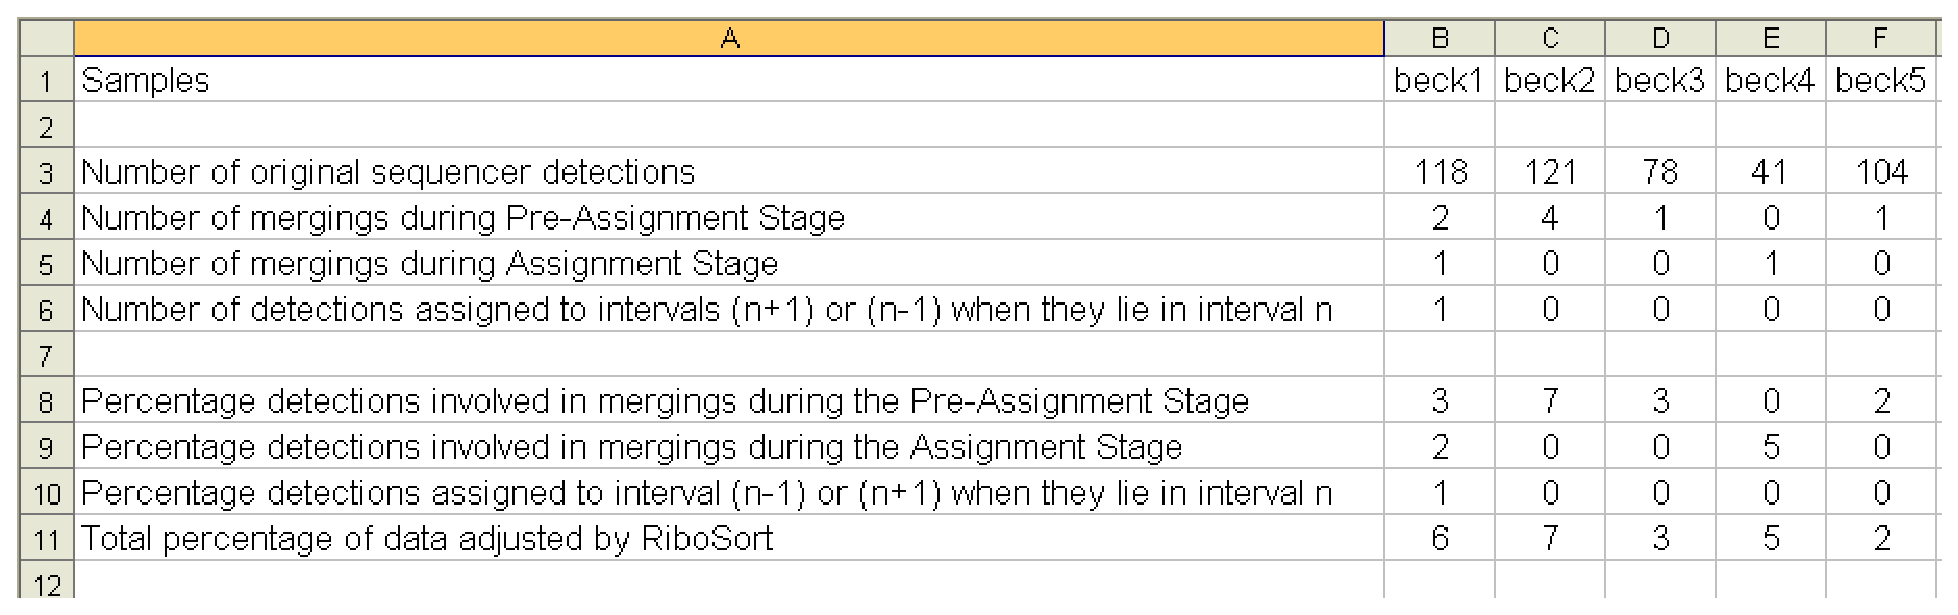
\includegraphics[width=0.9\textwidth,height=1.5in]{EPS/picinfo.eps}
\caption{An edited \textit{Information File.xls}.}
\label{fig:info}
\end{figure}

\begin{figure}
\centering
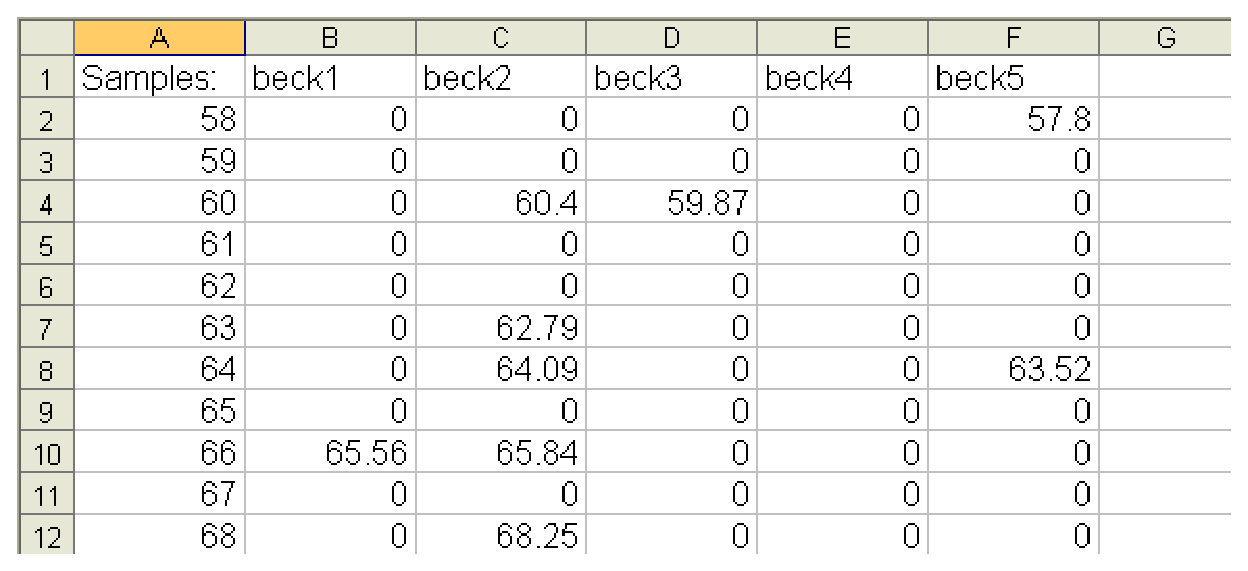
\includegraphics[width=0.8\textwidth,height=2in]{EPS/picribo.eps}
\caption{An edited \textit{Ribotypes Output.xls} file.}
\label{fig:ribo}
\end{figure}

\begin{figure}
\centering
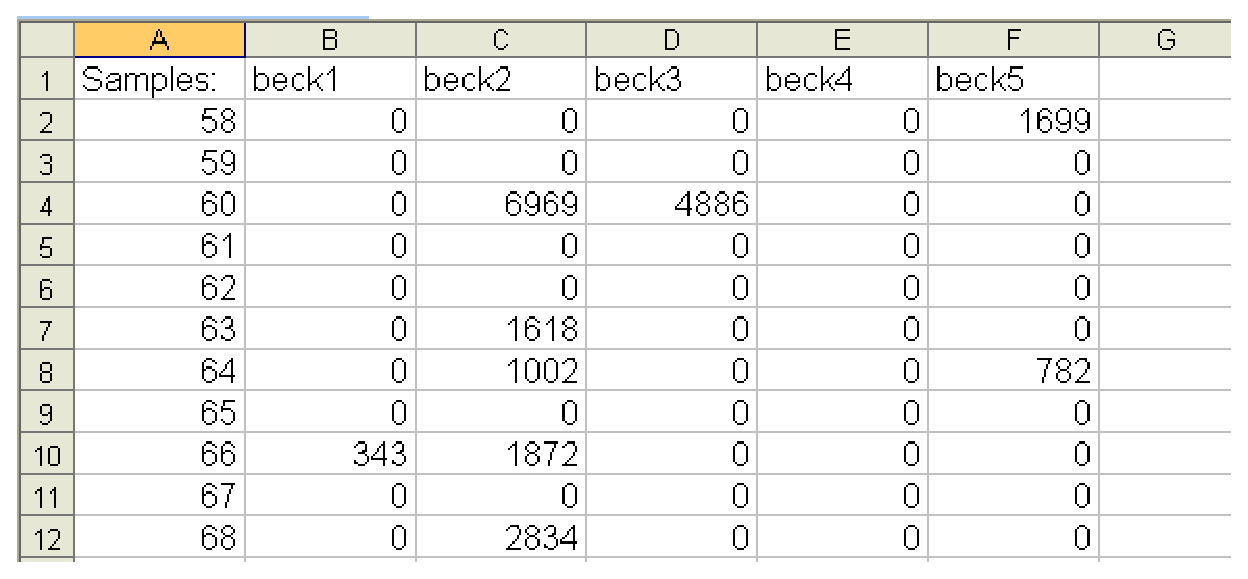
\includegraphics[width=0.8\textwidth,height=2in]{EPS/picabund.eps}
\caption{An edited \textit{Abundances Output.xls} file.}
\label{fig:abund}
\end{figure}

\begin{figure}
\centering
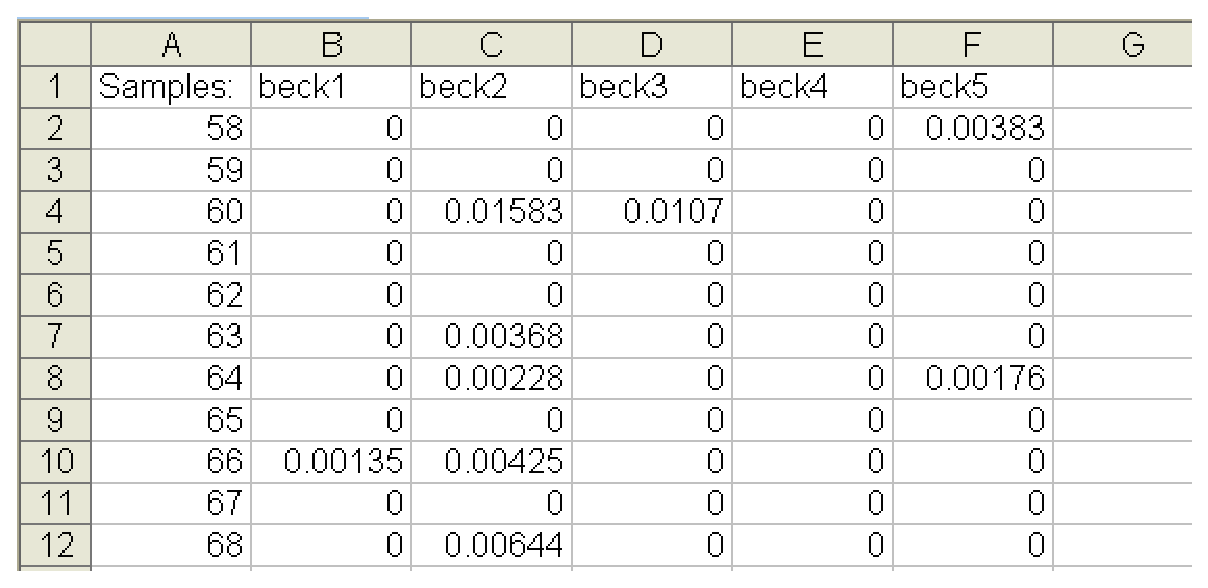
\includegraphics[width=0.8\textwidth,height=2in]{EPS/picprop.eps}
\caption{An edited \textit{Proportions Output.xls} file.}
\label{fig:prop}
\end{figure}

\section{Using RiboSort Results}

A RiboSort object (that is the object created in R by running the RiboSort function) is a matrix with columns representing samples and rows representing ribotypes (putative species). Although an Excel file containing this matrix is created by the RiboSort function ({\em Abundances Output.xls} if \texttt{output}=\texttt{"abundances"} or {\em Proportions Output.xls} if \texttt{output}=\texttt{"proportions"}), the function also stores the matrix as an R object to facilitate further  analysis in the R environment.

The RiboSort package has two functions \texttt{samplesMDS} and \texttt{speciesMDS} that produce multi-dimensional scalling (MDS) plots of samples and species respectively. These functions enable simple and quick production of multi-dimensional scaling plots. They each take four arguments that work as a interactive tools, allowing the user to personalize the plots.  A choice of dissimilarities is available, as well as the option to specify the desired type of multi-dimensional scaling. See the help file \texttt{?sampleMDS} for more information.

Note that at least three samples are required to produce a two-dimensional plot. The complete functions are demonstrated below, with each argument set to its default value.

\begin{Schunk}
\begin{Sinput}
> samplesMDS(x, dissimilarity = "euclidean", type = "non-metric", 
+     labels = TRUE)
> speciesMDS(x, dissimilarity = "euclidean", type = "non-metric", 
+     labels = TRUE)
\end{Sinput}
\end{Schunk}
We now proceed to describe the purpose of each argument and their associated options.

\begin{description}
\item[\texttt{x}] A numeric matrix, dataframe or a \texttt{RiboSort} object, ie. an object created by the \texttt{RiboSort} function.
\item[\texttt{dissimilarity}] The distance measure to be used computing dissimilarities between samples or species. This must be one of \texttt{"euclidean"}, \texttt{"maximum"}, \texttt{"manhattan"}, \texttt{"canberra"}, \texttt{"binary"} or \texttt{"minkowski"}. Any unambiguous substring can be given.
\item[\texttt{type}] The type of Multi-dimensional Scaling to be used. This must be one of \texttt{"classical"}, \texttt{"sammon"} or \texttt{"non-metric"}, the default.
\item[\texttt{labels}] An logical argument indicating whether or not labels are to be included on the MDS plot. When FALSE, labels are omitted.
\end{description}
%
When deciding upon a dissimilarity measure, the following description (available in the help file \texttt{?dist}) of options may aid your choice. Available dissimilarity measures are (written for two vectors x and y):
%
\begin{description}
\item [\texttt{euclidean}] Usual square distance between the two vectors.
\item [\texttt{maximum}] Maximum distance between two components of x and y.
\item [\texttt{manhattan}] Absolute distance between the two vectors.
\item [\texttt{canberra}] sum($|x_{i} - y_{i}| / |x_{i} + y_{i}|$). Terms with zero numerator and denominator are omitted from the sum and treated as if the values were missing.
\item [\texttt{binary}] The vectors are regarded as binary bits, so non-zero elements are 'on' and zero elements are 'off'. The distance is the \textit{proportion} of bits in which only one is on amongst those in which at least one is on.
\item [\texttt{minkowski}] The p norm, the pth root of the sum of the pth powers of the differences of the components.
\end{description}
%
When choosing which type of multi-dimensional scaling to use, the following elaboration on the options available may aid your choice.
%
\begin{description}
\item [\texttt{classical}] Classical multi-dimensional scaling of a data matrix. Also known as principal coordinates analysis.
\item [\texttt{sammon}] Sammon's non-linear mapping, also known as metric least squares  multi-dimensional scaling.
\item [\texttt{non-metric}] Kruskal's form of non-metric multidimensional scaling.
\end{description}
%
\vspace{3mm}
\textbf{Example:}\\
Let \texttt{x} be a RiboSort object. This example shows how an MDS plot for four samples, generated by the Beckman Coulter sequencer, is produced. The plot, illustrated in Figure~\ref{fig:beck14}, is created using non-metric multi-dimensional scaling on a dissimilarity matrix of euclidean distances.

\begin{Schunk}
\begin{Sinput}
> mydata = c("beck1.txt", "beck2.txt", "beck3.txt", "beck4.txt")
> x = RiboSort(data = mydata, dataformat = "beckman", dye = "D4")
> samplesMDS(x, dissimilarity = "euclidean", type = "non-metric", 
+     labels = TRUE)
\end{Sinput}
\end{Schunk}
\begin{figure}
\centering
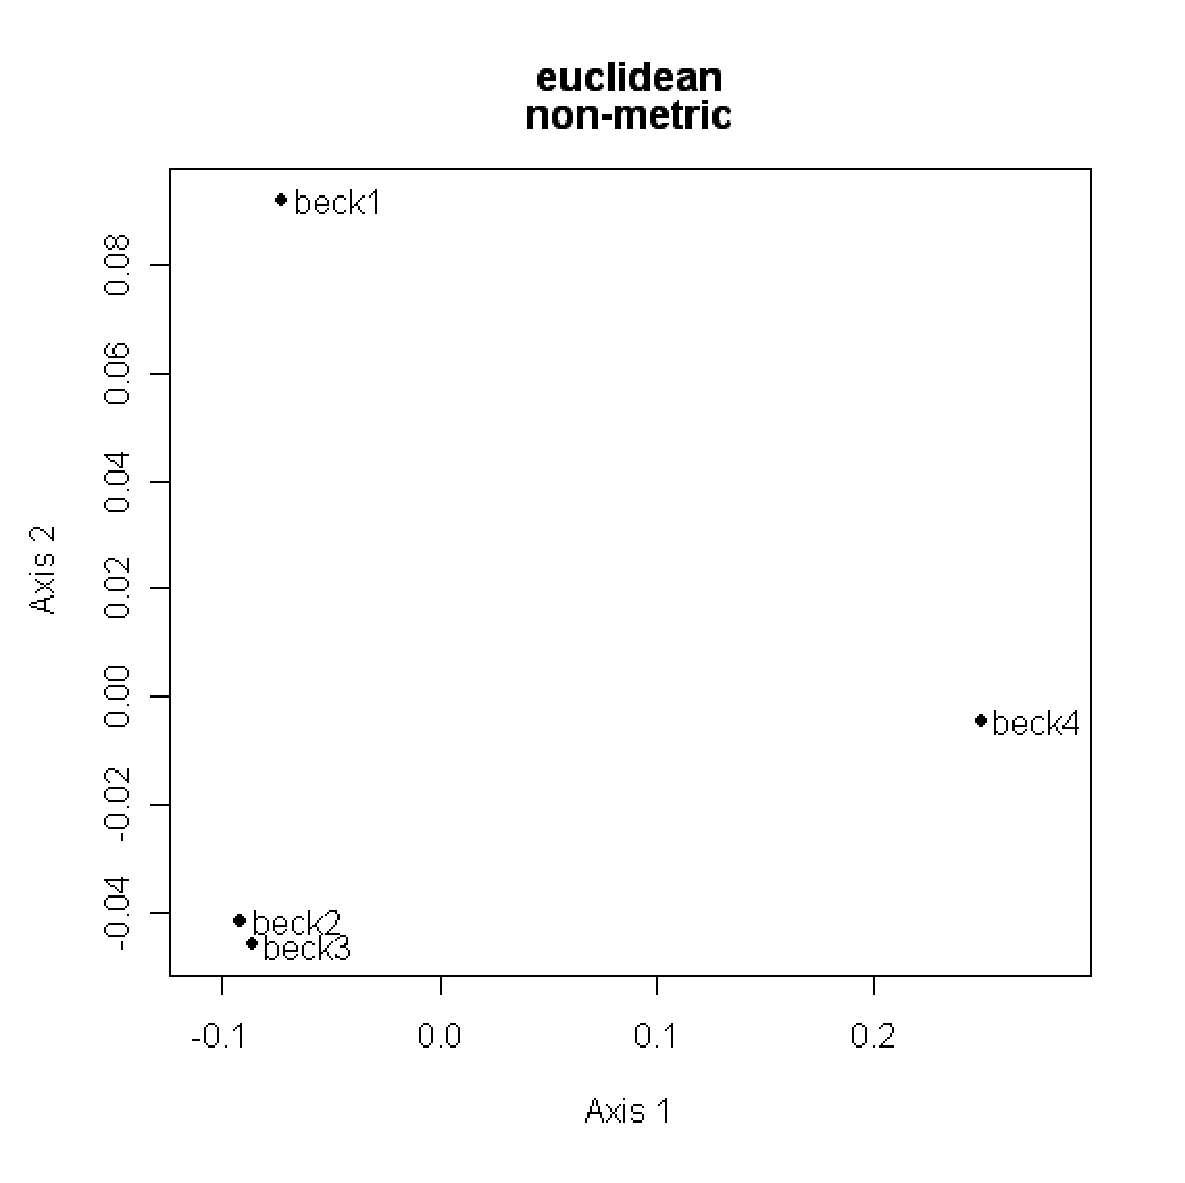
\includegraphics[height=3in]{EPS/beck14mdsplot.eps}
\caption{An MDS plot of four samples.}
\label{fig:beck14}
\end{figure}

Note that arguments left unspecified are evaluated at their default values. The following two lines of code are therefore equivalent.

\begin{Schunk}
\begin{Sinput}
> x = RiboSort(data = mydata, dataformat = "beckman", dye = "D4")
> x = RiboSort(data = mydata, dataformat = "beckman", dye = "D4", 
+     output = "proportions", zerorows = FALSE, repeats = 1, mergerepeats = "none")
\end{Sinput}
\end{Schunk}
For a more interactive and less limited approach to producing multi-dimensional scaling graphs, see the help files for the following functions: \texttt{cmdscale}, \texttt{sammon}, \texttt{isoMDS}.


\section{Appendix 1: Getting Started in R}
\subsection{Installation of R Software}
\begin{itemize}
\item Go to http://cran.r-project.org/.
\item In the Download and Install R box, select the operating system appropriate to your workstation. If your operating system is Windows, proceed to follow the remaining instructions outlined below. Linux and MacOS~X users should at this point, choose the latest version of R to download.
\item Enter the \texttt{base} subdirectory. To download the latest version of R, click on R-\ldots-win32.exe. Save this application and upon completion of the download, open it. This activates the R for Windows Setup Wizard. Follow the Wizard instructions. On the select components page, leave default settings in place. Tick the box to create a shortcut on your desktop.
\end{itemize}

\subsection{Intalling the RiboSort Package}
\begin{itemize}
\item Go to http://cran.r-project.org/.
\item Enter Packages under the Software heading on the left hand side. Scroll down to Available Packages and Bundles. Browse the list and enter the RiboSort link.
\item Download the appropriate file for your operating system. If working in Windows, right-click on the \textit{.zip} file and select \textit{Save Target as\ldots} Save the file in the library subdirectory of R (usually located at C:/Program Files/R/R-2.4.1/library).
\item Now start R from the desktop icon. On the top menu, enter {\em Packages $\rightarrow$ Install packages from local zip files\ldots} The package is now installed and ready for use in R.
\end{itemize}

\subsection{Brief explanation of How R works}
The R environment is an integrated suite of software facilities for data manipulation, calculation and graphical display. R is an interpreted language, not a compiled one, meaning that all commands submitted are directly executed without the requirement of building a complete program like in most computer languages. 

When R is opened on your computer, the R console will appear. This issues a prompt when it expects input commands. The default prompt is >. Commands can be input directly into the console. Generally, multiple commands are written in a script file and then submitted simultaneously to the console. To open a script file, go to the top menu and select {\em File $\rightarrow$ Open Script}. Frequently, an entire program is saved in a script file. To submit code in a script file to the R console, simply highlight the desired code and right-click {\em Run line or selection}. Errors in code are communicated via error messages in the console. These messages appear in blue font, making them easily distinguishable from successfully executed code which appears in red.

Help is available through R via the top menu. The \textit{Manuals (in PDF)} option provides seven manuals that comprehensively document R's functionality. In particular, An Introduction to R introduces the language and explains how to use R for statistical analysis and graphics. All R objects (including functions, datasets, packages, etc.) have associated documentation files. These can be accessed via the R console by typing a question mark followed by the name of the object. For example, submit \texttt{?sum} to your R console. Note the vast index of documented objects that appears on the left hand side.

\subsection{The Working Directory}
All files that are to be imported (used) by R must be stored in the current working directory. Files created by R are also stored in this directory. It is recommended to use different working directories for different projects you are working on. There are two ways to set up a working directory:
\begin{description}
\item[Method 1]
Right-click on the R shortcut displayed on your desktop and enter Properties. The Start In field contains the path to the current working directory. To change working directory, simply change the path so that it refers to the desired folder. All files to be used by R must be stored in this folder, and any output files created by R will also be stored in this folder.
\item[Method 2]
Establish the current working directory by submitting the following code. To do this type \texttt{getwd()} in the R console and press enter.

\begin{Schunk}
\begin{Sinput}
> getwd()
\end{Sinput}
\end{Schunk}
To change the working directory submit the code below inserting the path to the folder you wish to use as your working directory within the inverted commas. Forward slashes as opposed to backslashes must be used in the path name.

\begin{Schunk}
\begin{Sinput}
> setwd("C:/uscallan/myRiboSortfolder")
\end{Sinput}
\end{Schunk}
To confirm the change of directory, resubmit getwd(). 
\end{description}

\end{document}
